% !TeX spellcheck = en_GB
\documentclass[aspectratio=169]{beamer}

%\usepackage[utf8]{inputenc}
%\usepackage[T1]{fontenc}
%\usepackage{lmodern}
\usepackage{fontspec}
\usepackage[english]{babel}
\usepackage{amsmath}
\usepackage{amsfonts}
\usepackage{amssymb}
\usepackage{graphicx}
\usepackage{bigints}
\usepackage{verbatim}
\usepackage{caption}
\usepackage[export]{adjustbox}
\usepackage[backend=bibtex,style=numeric]{biblatex}

\bibliography{String_Theory.bib}

\usetheme{Madrid}

\usefonttheme{professionalfonts}

\setbeamertemplate{itemize item}[triangle]
\setbeamertemplate{itemize subsubitem}[square]
\setbeamertemplate{enumerate item}[default]
\setbeamertemplate{enumerate subitem}[default]
\setbeamertemplate{bibliography item}{\insertbiblabel}

\begin{document}	
	\author{Mate Zoltan Farkas}
	\title{An Introduction to String Theory}
	%\subtitle{}
	%\logo{}
	%\institute{}
	%\date{}
	%\subject{}
	\setbeamercovered{transparent}
	\setbeamertemplate{navigation symbols}{}
	
	\begin{frame}[plain]
		\maketitle
	\end{frame}
	
	\begin{frame}
		\frametitle{Table of Contents}
		\tableofcontents
	\end{frame}

	\section{Introduction}
	\subsection{Notation}
	
	\begin{frame}
		\frametitle{Introduction -- Notation}
		\begin{itemize}
			\item Metric:
			\begin{itemize}
				\item $\eta_{\mu\nu}$ = diag(-1,+1, $\dots$, +1)
			\end{itemize}
		\end{itemize}
	\end{frame}

	\section{The Relativistic String}
	\subsection{The Relativistic Point Particle}
	
	\begin{frame}
		\frametitle{The Relativistic Point Particle -- The Action}
		\begin{itemize}[]
			\item<1-> Consider the action of a point particle (with fixed coordinates $X_\mu = (t,\vec{x})$ in a given frame):
			\begin{equation*}
				S = -m \int dt \, \sqrt{1-\dot{\vec{x}}\dot{\vec{x}}}
			\end{equation*}
			\item<1->[] $\rightarrow$ not Lorentz-invariant, due to mixture of spacial and temporal coordinates under a Lorentz-transformation $\Lambda$.
			\item[]
			\item<2-> Consider instead for a generalized coordinate $\tau$ along the line element:
			\begin{columns}
				\begin{column}{0.8\textwidth}
					\begin{equation*}
						S = -m \int d\tau \, \sqrt{-\frac{dX^\mu}{d\tau} \frac{dX^\nu}{d\tau}\eta_{\mu\nu}}
					\end{equation*}
				\end{column}
				\begin{column}{0.2\textwidth}
					\begin{figure}
						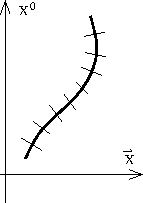
\includegraphics[width=0.5\linewidth]{res/TongP17_graph}
						\caption*{Ref: \cite{tong_lectures_2012}}
					\end{figure}
				\end{column}
			\end{columns}
			\item[]<2-> Remark: $S$ is proportional to the integral over the worldline of the particle
		\end{itemize}
	\end{frame}

	\subsection{Dynamics of a Relativistic String -- The Nambu-Goto Action}
	
	\begin{frame}[t]
		\frametitle{Dynamics of a Relativistic String -- The Nambu-Goto Action}
		Action of the Relativistic String?
		\begin{itemize}
			\item[]<only@1>
			\begin{center}
				\begin{tabular}{ccp{1.8cm}cc}
					particle & $\Leftrightarrow$ & worldline & $\Leftrightarrow$ & ${\displaystyle S = -m \int d\tau \,\sqrt{-\frac{dX^\mu}{d\tau} \frac{dX^\nu}{d\tau}\eta_{\mu\nu}} }$ \\
					&&&&\\
					closed string & $\Leftrightarrow$ &\hphantom{worl} ? \hphantom{heet}& $\Leftrightarrow$ & ? \\
				\end{tabular}
			\end{center}
			\item[]<only@2>
			\begin{center}
				\begin{tabular}{ccp{1.8cm}cc}
					particle & $\Leftrightarrow$ & worldline & $\Leftrightarrow$ & ${\displaystyle S = -m \int d\tau \,\sqrt{-\frac{dX^\mu}{d\tau} \frac{dX^\nu}{d\tau}\eta_{\mu\nu}} }$ \\
					&&&&\\
					closed string & $\Leftrightarrow$ & worldsheet & $\Leftrightarrow$ & ? \\
				\end{tabular}
			\end{center}
			\item[]<only@3>
			\begin{center}
				\begin{tabular}{ccp{1.8cm}cc}
					particle & $\Leftrightarrow$ & worldline & $\Leftrightarrow$ & ${\displaystyle S = -m \int d\tau \,\sqrt{-\frac{dX^\mu}{d\tau} \frac{dX^\nu}{d\tau}\eta_{\mu\nu}} }$ \\
					&&&&\\
					closed string & $\Leftrightarrow$ & worldsheet & $\Leftrightarrow$ & Nambu-Goto/Dirac Action \\
				\end{tabular}
			\end{center}
		\end{itemize}
	\end{frame}

	\begin{frame}
		\frametitle{The Relativistic Point Particle -- Action Symmetries}
		\begin{itemize}
			\item[]<1-> What are the symmetries of
			\begin{equation*}
				S = -m \int d\tau \, \sqrt{-\frac{dX^\mu}{d\tau} \frac{dX^\nu}{d\tau}\eta_{\mu\nu}}
			\end{equation*}
			\item<2-> Reparametrization invariance:
			\begin{flushleft}
				Let $\tilde{\tau} = \tilde{\tau}(\tau)$. Then:
				\begin{equation*}
					S' = -m \int d\tilde{\tau} \, \sqrt{-\frac{dX^\mu}{d\tilde{\tau}}\frac{dX^\nu}{d\tilde{\tau}}\eta_{\mu\nu}} = S
				\end{equation*}
				$\rightarrow$ gauge symmetry of the action $\rightarrow$ still D-1 dof!
			\end{flushleft}
			\item<2-> Poincaré invariance:
			\begin{flushleft}
				Let:
				\begin{equation*}
					X'^\mu = \Lambda^\mu{}_\nu X^\nu + c^\mu
				\end{equation*}
				Then:
				\begin{equation*}
					S'=S, \qquad \text{as} \qquad \Lambda^\mu{}_\rho \, \eta_{\mu\nu} \, \Lambda^\nu{}_\sigma = \eta_{\rho\sigma}
				\end{equation*}
			\end{flushleft}
		\end{itemize}
	\end{frame}
	
	\begin{frame}
		\frametitle{Never forget the Titles!}
		\begin{itemize}
			%\centering
			\item<1,2,3,4,5> first item 
			\begin{itemize}
				\item<2,3,4,5> subitem
				\begin{itemize}
					\item<3,4,5> subsubitem
				\end{itemize}
			\end{itemize}
			\item<4,5>second item
			\begin{enumerate}
				\item item 1
				\begin{enumerate}
					\item subitem 1
					\item subitem 2
				\end{enumerate}
				\item item 2
			\end{enumerate}
			\item<5>third item
		\end{itemize}	
	\end{frame}

	\section{Covariant Quantization of the Solutions}
	
	\begin{frame}
		\frametitle{Covariant Quantization of the Solutions of the Nambu-Goto Action}
		
		\begin{equation}
			S = \frac{1}{2\pi\alpha'}\int\sqrt{-\det g} \, \partial_\mu
		\end{equation}
	
	\end{frame}	

	\section{Quantization in the Lightcone Gauge}
	
	\begin{frame}
		\frametitle{Quantization of $X^\mu$ in the Lightcone Gauge}
	\end{frame}

	\begin{frame}
		\frametitle{References}
		\printbibliography
	\end{frame}

\end{document}